%% bare_jrnl_compsoc.tex
%% V1.4a
%% 2014/09/17
%% by Michael Shell
%% See:
%% http://www.michaelshell.org/
%% for current contact information.
%%
%% This is a skeleton file demonstrating the use of IEEEtran.cls
%% (requires IEEEtran.cls version 1.8a or later) with an IEEE
%% Computer Society journal paper.
%%
%% Support sites:
%% http://www.michaelshell.org/tex/ieeetran/
%% http://www.ctan.org/tex-archive/macros/latex/contrib/IEEEtran/
%% and
%% http://www.ieee.org/

%%*************************************************************************
%% Legal Notice:
%% This code is offered as-is without any warranty either expressed or
%% implied; without even the implied warranty of MERCHANTABILITY or
%% FITNESS FOR A PARTICULAR PURPOSE! 
%% User assumes all risk.
%% In no event shall IEEE or any contributor to this code be liable for
%% any damages or losses, including, but not limited to, incidental,
%% consequential, or any other damages, resulting from the use or misuse
%% of any information contained here.
%%
%% All comments are the opinions of their respective authors and are not
%% necessarily endorsed by the IEEE.
%%
%% This work is distributed under the LaTeX Project Public License (LPPL)
%% ( http://www.latex-project.org/ ) version 1.3, and may be freely used,
%% distributed and modified. A copy of the LPPL, version 1.3, is included
%% in the base LaTeX documentation of all distributions of LaTeX released
%% 2003/12/01 or later.
%% Retain all contribution notices and credits.
%% ** Modified files should be clearly indicated as such, including  **
%% ** renaming them and changing author support contact information. **
%%
%% File list of work: IEEEtran.cls, IEEEtran_HOWTO.pdf, bare_adv.tex,
%%                    bare_conf.tex, bare_jrnl.tex, bare_conf_compsoc.tex,
%%                    bare_jrnl_compsoc.tex, bare_jrnl_transmag.tex
%%*************************************************************************

% *** Authors should verify (and, if needed, correct) their LaTeX system  ***
% *** with the testflow diagnostic prior to trusting their LaTeX platform ***
% *** with production work. IEEE's font choices and paper sizes can       ***
% *** trigger bugs that do not appear when using other class files.       ***                          ***
% The testflow support page is at:
% http://www.michaelshell.org/tex/testflow/

\documentclass[10pt,conference,onecolumn,compsoc]{IEEEtran}

\usepackage{hyperref}
\usepackage{enumitem}
\setlist[itemize]{leftmargin=3 cm}
\setlist[enumerate]{leftmargin=3cm}

% *** CITATION PACKAGES ***
%
\ifCLASSOPTIONcompsoc
  % IEEE Computer Society needs nocompress option
  % requires cite.sty v4.0 or later (November 2003)
  \usepackage[nocompress]{cite}
\else
  % normal IEEE
  \usepackage{cite}
\fi
% cite.sty was written by Donald Arseneau
% V1.6 and later of IEEEtran pre-defines the format of the cite.sty package
% \cite{} output to follow that of IEEE. Loading the cite package will
% result in citation numbers being automatically sorted and properly
% "compressed/ranged". e.g., [1], [9], [2], [7], [5], [6] without using
% cite.sty will become [1], [2], [5]--[7], [9] using cite.sty. cite.sty's
% \cite will automatically add leading space, if needed. Use cite.sty's
% noadjust option (cite.sty V3.8 and later) if you want to turn this off
% such as if a citation ever needs to be enclosed in parenthesis.
% cite.sty is already installed on most LaTeX systems. Be sure and use
% version 5.0 (2009-03-20) and later if using hyperref.sty.
% The latest version can be obtained at:
% http://www.ctan.org/tex-archive/macros/latex/contrib/cite/
% The documentation is contained in the cite.sty file itself.

% *** GRAPHICS RELATED PACKAGES ***
%
\ifCLASSINFOpdf
   \usepackage[pdftex]{graphicx}
 
\else
 
\fi
% graphicx was written by David Carlisle and Sebastian Rahtz. It is
% required if you want graphics, photos, etc. graphicx.sty is already
% installed on most LaTeX systems. The latest version and documentation
% can be obtained at: 
% http://www.ctan.org/tex-archive/macros/latex/required/graphics/
% Another good source of documentation is "Using Imported Graphics in
% LaTeX2e" by Keith Reckdahl which can be found at:
% http://www.ctan.org/tex-archive/info/epslatex/
%
% latex, and pdflatex in dvi mode, support graphics in encapsulated
% postscript (.eps) format. pdflatex in pdf mode supports graphics
% in .pdf, .jpeg, .png and .mps (metapost) formats. Users should ensure
% that all non-photo figures use a vector format (.eps, .pdf, .mps) and
% not a bitmapped formats (.jpeg, .png). IEEE frowns on bitmapped formats
% which can result in "jaggedy"/blurry rendering of lines and letters as
% well as large increases in file sizes.
%
% You can find documentation about the pdfTeX application at:
% http://www.tug.org/applications/pdftex

% *** PDF, URL AND HYPERLINK PACKAGES ***
%
\usepackage{url}
% url.sty was written by Donald Arseneau. It provides better support for
% handling and breaking URLs. url.sty is already installed on most LaTeX
% systems. The latest version and documentation can be obtained at:
% http://www.ctan.org/tex-archive/macros/latex/contrib/url/
% Basically, \url{my_url_here}.

\usepackage{fancyvrb}
%              --------------------------------------------------
%              |                   `fancyvrb'                   |
%              |                                                |
%              | Timothy Van Zandt (Princeton University - USA) |
%              |                                                |
%              |     Packaging, documentation and support       |
%              |       Denis Girou (CNRS/IDRIS - France)        |
%              |            <Denis.Girou@idris.fr>              |
%              |        Sebastian Rahtz (Elsevier - GB)         |
%              |       Herbert Voss, Berlin (hvoss@tug.org)     |
%              --------------------------------------------------
%% This package may be distributed under the terms of the LaTeX Project Public
%% License, as described in lppl.txt in the base LaTeX distribution.
%% Either version 1.3 or, at your option, any later version.

% ************************************************************************************** %
% END LEGAL DISCLAIMERS & CREDITS
% ************************************************************************************** %




\begin{document}

% Title
\begin{figure}

% Splash Art
\centering
\begin{footnotesize}
\begin{BVerbatim}
 .d8888b. Y88b   d88P 888888b.   8888888888 8888888b.  888b    888 888    888 888    d8P  8888888888 
d88P  Y88b Y88b d88P  888  "88b  888        888   Y88b 8888b   888 888    888 888   d8P   888        
888    888  Y88o88P   888  .88P  888        888    888 88888b  888 888    888 888  d8P    888        
888          Y888P    8888888K.  8888888    888   d88P 888Y88b 888 888    888 888d88K     8888888    
888           888     888  "Y88b 888        8888888P"  888 Y88b888 888    888 8888888b    888        
888    888    888     888    888 888        888 T88b   888  Y88888 888    888 888  Y88b   888        
Y88b  d88P    888     888   d88P 888        888  T88b  888   Y8888 Y88b..d88P 888   Y88b  888        
 "Y8888P"     888     8888888P"  8888888888 888   T88b 888    Y888  "Y8888P"  888    Y88b 8888888888 
<><><><><><><><><><><><><><><><><><><><><><><><><><><><><><><><><><><><><><><><><><><><><><><><><><>

\end{BVerbatim}
\end{footnotesize}

% Title, Sub-title, Authors
CYBERNUKE\\
{\small POST-APOCALYPTIC CYBERPUNK ROGUELIKE}\\
J. Kenneth Wallace, Vance Brender-A-Brandis\\
\end{figure}

% Old Title, Authors
%\title{{\Huge CYBERNUKE}\\Post-Apocalyptic Cyberpunk Roguelite}
%\author{J. Kenneth Wallace, Vance Brenderabrandis\\}

% Abstract
\IEEEtitleabstractindextext{
\begin{abstract}
CYBERNUKE is a roguelite game developed in the C\# WPF format. You play as an amnesiac cyborg who awakens in the middle of a destroyed futuristic city and must discover who they were and what happened to them. The game combines a post-apocalyptic and cyberpunk setting to create a distinct atmosphere not previously explored by other games. The setting of the game is inspired by popular stories such as \emph{Fallout}, \emph{Cyberpunk 2077}, and other games like \emph{FTL: Faster than Light} and the \emph{Megami Tensei} series.
\end{abstract}
}


% Title Area
%\maketitle
\IEEEdisplaynontitleabstractindextext
\IEEEpeerreviewmaketitle



% INTRODUCTION ************************************************************************* %
\section{Introduction}

For this project we aim to create a roguelike to gain some experience with C\#, WPF, and game design. With CYBERNUKE, we're trying to showcase our understanding of the Cyberpunk and Post-apocalyptic genres by creating a unique setting that blends both ideas together. Our target audience is primarily those who enjoy roguelikes but would like to experience a new  and unique setting. 

For reference, Cyberpunk is a \emph{"science-fiction subgenre characterized by countercultural antiheroes trapped in a dehumanized, high-tech future"}\cite{IEEEhowto:cyberpunk} and roguelites are \emph{"a subgenre of roguelikes that has most of the game design philosophies of roguelikes, but also has at least one progression element that persists after failure"}\cite{IEEEhowto:roguelite_1}. Essentially, this means that whenever the player fails a run (either by their player dying or some other failure condition), the player must restart but with some form of saved progress such that they are not starting from zero. 

Mixed together with this game genre is the post-apocalyptic setting seen in popular games such as \emph{Fallout}, \emph{Wasteland}, and \emph{Metro}. Although broad, the post-apocalyptic genre is defined by a setting where nuclear warfare, or any disaster, has caused modern society to collapse. We believe that a blend of these two settings can create an interesting theme for our game that hasn't been explored by others.

This game's estimated impact is very low. An optimistic prediction would be that our game reaches a larger audience and inspires others to create roguelikes or other games with a similar setting to ours. Other than that, we hope to entertain at least one person with our game.

One of the most difficult challenges we face right now is our lack of experience not only with C\# and WPF, but also with game design in general. For example, goals such as movement, combat, stats, and so forth will all have to be developed and implemented without any prior knowledge of how to do these things. However, inexperience is a treatable disease. We have access to a plethora of online resources that we can study and use to create this project, and we will do so. 

%Your introduction should give an introduction to your project.  What are you trying to accomplish (high level), who do you expect to target with your project?  What do you expect your target audience will get out of it?
%Should you need to cite anything, use the \emph{cite} keyword, and refer to something from your bibliography.  For example, this was put together with the help of a \LaTeX guide\cite{IEEEhowto:kopka}.
%Make sure that by the end of your introduction the reader knows what your project is and why you are doing it.

\subsection{Audience}
CYBERNUKE's target audience is those who enjoy playing RPGs and roguelites but are looking for a fresh new setting. We also hope to appeal to fans of the cyberpunk and post-apocalyptic genres who have never played a roguelite before. 

\pagebreak
\subsection{Background}
We chose to make a game for our project because it is a genre in which we are both very familiar. A game is also much more enjoyable to create and play than a calculator or calendar app. CYBERNUKE is a roguelite game, which is a subset of roguelike games. The most widely accepted definition is the Berlin Interpretation, which was developed at the 2008 International Roguelike Development Conference.\cite{IEEEhowto:roguelite_2} It says that all roguelikes must have these features:
\begin{enumerate}
\item Permadeath
\item Random environment generation
\item Exploration and discovery
\item Turn-based, grid-based, non-modal gameplay
\item Hack-n-slash
\item Resource management
\end{enumerate}

CYBERNUKE is a roguelite as it only includes some of these features, like exploration \& discovery, turn-based \& grid-based gameplay, and resource management.

The setting of CYBERNUKE is a blend between two popular genres: Cyberpunk and Post-apocalypse.  Cyberpunk is a \emph{"science-fiction subgenre characterized by countercultural antiheroes trapped in a dehumanized, high-tech future"}\cite{IEEEhowto:cyberpunk}; and Post-apocalypse is genre characterized by the collapse of society due to a disaster. We believe that we can create a new, unique setting for our game by blending these two genres together.

\subsection{Impacts}
We believe that the overall impact of this game will be minimal. An optimistic estimate would be that when our game is released, it will reach a larger audience that will play, discuss, and enjoy it. If this is the case, it may inspire others to create games or stories with a setting similar to CYBERNUKE.

\subsection{Challenges}
Going into this, we have a lot of challenges to face. One of the most significant is that we have almost no experience working with C\#, WPF, or in game design. If we are to complete CYBERNUKE within the time frame, we will need a lot of reference material. We believe it is doable though. 
Apart from getting used to WPF, there is no "most difficult" part that we can think of. All of the core mechanics that must be added will be difficult, some more than others; however, we lack the experience to differentiate the difficulty of each implementation. 



%\pagebreak
% SCOPE ******************************************************************************** %
\section{Scope}
In order of importance, these are the fundamental game mechanics that must be implemented for \emph{CYBERNUKE} to be considered functional:
\begin{enumerate}
\item Operational Interfaces (Main Menu, Option Menu)
\item Maps
\item User Interface (Map Screen, Player HUD)
\item Character Movement, Interaction
\item Character Interface (Name, Stats)
\item Enemies, Enemy Encounters
\item Combat, Combat Interface
\item Player Saves \& Load Menu
\end{enumerate} 

\begin{flushleft}
1. The Operational Interfaces are the menus that are used to interact with the game when the player is not playing the game (Main Menu, Option Menu).

2. The maps are pre-made rather than generated automatically; in this case, it will only be a simple testing map until later.

3. The User Interface includes the Map Screen, which renders the current map to the screen. The Player HUD displays the player's statistics such as Hit Points, Money, and so on.

4. Character Movement refers to moving around the map with the player character. Character Interaction refers to how the player interacts with the map, such as unlocking locked doors or moving between maps.

5. Character Interface differs from User Interface in that it is a separate menu that displays the character's full stats such as HP, Strength, Luck, Agility, and so on, as well as their name.

6. Enemies are the monsters/humans that the player will encounter throughout the game. Enemy Encounters refers to how you will find monsters in the first place, which is primarily done through a "percent encounter" system akin to the old \textit{Pokemon} games. There may also be opportunities for pre-scripted encounters.

7. Combat refers to fights between the player character and enemies in this game, which will be turn-based. Actual combat is made possible by the Combat Interface.

8. Players can save their state (at specific points in the game) and load back in at a later time using Player Saves and the Load Menu.
\end{flushleft}

After the fundamental game mechanics are in place, additional features that flesh out the game can be added.

Possible stretch-goal features (In no particular order):
\begin{enumerate}
\item Companions and Party System
\item Hacking Puzzles
\item More Enemy Types
\item More Story Content
\item Items, Loot, Weapons, Armor, etc.
\item Cybernetic Augmentation
\item Leveling System
\item Currency and Merchants
\item Expanded Character Creation (Species, Backstory, etc.)
\end{enumerate}


%This section is a bit tricksy.  You are going to do your best to set up ground rules:  How will you know when your project is done?
%If you were doing this under contract for a company, this would be your checklist to make sure you get paid.  We will be going into this in more detail over time, but you should start planning your major goals of the project as soon as possible.
%For every sub(sub)section below, make sure to mark which items are basic goals (project won't be done without it) and which ones are stretch goals (it would be really cool to do...).  We will be meeting one-on-one to help identify which goals go where.


%pagebreak as it is not required for first deliverable
\pagebreak
\subsection{Requirements}
As part of fleshing out the scope of your requirements, you'll also need to keep in mind both your functional and non-functional requirements.  These should be listed, and explained in detail as necessary.  Use this area to explain how you gathered these requirements.

\subsubsection{Functional}
\begin{itemize}
\item User needs to have a private shopping cart -- this cannot be shared between users, and needs to maintain state across subsequent visits to the site
\item Users need to have website accounts -- this will help track recent purchases, keep shopping cart records, etc.
\item You'll need more than 2 of these...
\end{itemize}

\subsubsection{Non-Functional}
\begin{itemize}
\item Security -- user credentials must be encrypted on disk, users should be able to reset their passwords if forgotten
\item you'll typically have fewer non-functional than functional requirements
\end{itemize}

\subsection{Use Cases}
This subsection is arguably part of how you define your project scope (why it is in the Scope section...).  In a traditional Waterfall approach, as part of your requirements gathering phase (what does the product actually \emph{need} to do?), you will typically sit down with a user to develop use cases.

You should have a table listing all use cases discussed in the document, the ID is just the order it is listed in, the name should be indicative of what should happen, the primary actor is typically most important in an application where you may have different levels of users (think admin vs normal user), complexity is a best-guess on your part as to how hard it should be.  A lower number in priority indicates that it needs to happen sooner rather than later.  A sample table, or Use Case Index can be seen in Table \ref{tab:useCaseIndex}.




\begin{table}
\centering
\begin{tabular}{|c|c|c|c|c|}
\hline
Use Case ID & Use Case Name & Primary Actor & Complexity & Priority \\
\hline \hline
1 & Add item to cart & Shopper & Med & 1\\
\hline
2 & Checkout & Shopper & Med & 1\\
\hline

\end{tabular}
\caption{Sample use case table}
\label{tab:useCaseIndex}
\end{table}


\begin{itemize}
\item[Use Case Number:] 1
\item[Use Case Name:] Add item to cart
\item[Description:] A shopper on our site has identified an item they wish to buy.  They will click on a ``Add to Cart" button.  This will kick off a process to add one instance of the item to their cart.
\end{itemize}

You will then go on to (minimally) discuss a basic flow for the process:

\begin{enumerate}
\item User navigates to page listing desired item
\item User left-clicks on ``Add to Cart" button.
\item User cart is updated to reflect the new item, this also updates the current total.
\item[Termination Outcome:] The user now has a single instance of the item in their cart.
\end{enumerate}

You may need to also add in any alternative flows:

Alternative: Item already exists in the cart
\begin{enumerate}
\item User navigates to page listing desired item
\item User left-clicks on ``Add to Cart" button.
\item User cart is updated to reflect the new item, showing that one more instance of the existing item has been added.  This also updates the current total.
\item[Termination Outcome:] The user now has multiple instances of the item in their cart.
\end{enumerate}

You will often also need to include pictures or diagrams.  It is quite common to see use-case diagrams in such write-ups.  To properly reference an image, you will need to use the \texttt{figure} environment and will need to reference it in your text (via the \texttt{ref} command) (see Figure \ref{capybara1}).  NOTE: this is not a use case diagram, but a capybara.

After fully describing a use case, it is time to move on to the next use case:

\begin{itemize}
\item[Use Case Number:] 2
\item[Use Case Name:] Checkout
\item[Description:] A shopper on our site has finished shopping.  They will click on a ``Checkout" button.  This will kick off a process to calculate cart total, any taxes, shipping rates, and collect payment from the shopper.

\end{itemize}

You will then need to continue to flesh out all use cases you have identified for your project.

\begin{figure}[ht!]

\includegraphics[height=250px, width=350px]{capybara1.jpg}
\caption{First picture, look at the capybara}
\label{capybara1}
\end{figure}

\subsection{Interface Mockups}
At first, this will largely be completely made up, as you get further along in your project, and closer to a final product, this will typically become simple screenshots of your running application.

In this subsection, you will be showing what the screen should look like as the user moves through various use cases (make sure to tie the interface mockups back to the specific use cases they illustrate).



% PROJECT TIMELINE ********************************************************************* %
\section{Project Timeline}
Go back to your notes and look up a typical project development life cycle for the Waterfall approach.  How will you follow this life cycle over the remainder of this semester?  This will usually involve a chart showing your proposed timeline, with specific milestones plotted out.  Make sure you have deliverable dates from the course schedule listed, with a plan to meet them (NOTE: these are generally optimistic deadlines).



% PROJECT STRUCTURE ******************************************************************** %
\section{Project Structure}
At first, this will be a little empty (it will need to be filled in by the time you turn in your final report).  This is your chance to discuss all of your design decisions (consider this the README's big brother).

\subsection{UML Outline}
Show the full structure of your program.  Make sure to keep on updating this section as your project evolves (you often start out with one plan, but end up modifying things as you move along).  As a note, while Dia fails miserably at generating pdfs (probably my fault), I have had much success with png files.  Make sure to wrap your images in a \texttt{figure} environment, and to reference with the \texttt{ref} command.  For example, see Figure \ref{capybara2}.

\begin{figure}[ht!]
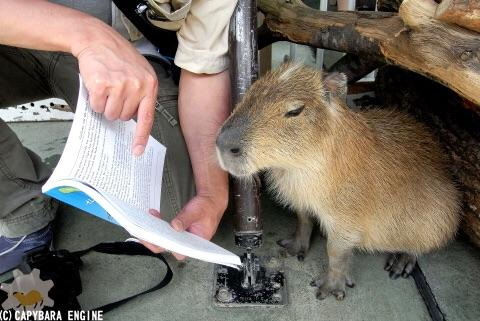
\includegraphics[scale=1]{capybara2.jpg}
\caption{Your figures should be in the \emph{figure} environment, and have captions.  Should also be of diagrams pertaining to your project, here we are teaching the capybaras to do our work.}
\label{capybara2}
\end{figure}


\subsection{Design Patterns Used}
Make sure to actually use at least 2 design patterns from this class.  This is not normally part of such documentation, but largely just specific to this class -- I want to see you use the patterns!



% RESULTS ****************************************************************************** %
\section{Results}
This section will start out a little vague, but it should grow as your project evolves.  With each deliverable you hand in, give me a final summary of where your project stands.  By the end, this should be a reflective section discussing how many of your original goals you managed to attain/how many desired use cases you implemented/how many extra features you added.

\subsection{Future Work}
Where are you going next with your project?
For early deliverables, what are your next steps?  (HINT: you will typically want to look back at your timeline and evaluate: did you meet your expected goals?  Are you ahead of schedule?  Did you decide to shift gears and implement a new feature?)
By the end, what do you plan on doing with this project?  Will you try to sell it?  Set it on fire?  Link to it on your resume and forget it exists?



% BIBLIOGRAPHY ************************************************************************* %
\bibliographystyle{IEEEtran}
\bibliography{./reference}

\begin{thebibliography}{1}

\bibitem{IEEEhowto:cyberpunk}
Britannica, T. Editors of Encyclopaedia. \emph{"cyberpunk."} Encyclopedia Britannica, 1999. https://www.britannica.com/art/cyberpunk.

\bibitem{IEEEhowto:roguelite_1}
Wiktionary. \emph{"roguelite"}
https://en.wiktionary.org/wiki/rogue-lite

\bibitem{IEEEhowto:roguelite_2}
whatNerd, Joel Lee. \emph{"What’s a Roguelike vs. Roguelite? Is the Difference Really That Important?"} whatNerd, 2021. https://whatnerd.com/what-is-a-roguelike-roguelite-difference/.

\end{thebibliography}

% END ********************************************************************************** %
\end{document}


